\documentclass[12pt, fleqn]{article}

\usepackage[utf8]{inputenc}
\usepackage[T2A]{fontenc}
\usepackage{amssymb,amsmath,mathrsfs,amsthm}
\usepackage[russian]{babel}
\usepackage{graphicx}
\graphicspath{ {../imgs/} }
\usepackage[footnotesize]{caption}
\usepackage{indentfirst}
\usepackage{amsthm}
\usepackage[font=small,labelfont=bf]{caption}
\usepackage[labelsep=space, singlelinecheck=on]{subcaption}

\usepackage{algorithm, setspace}
\usepackage{algpseudocode}
\usepackage[matrix,frame,arrow]{xy}
\usepackage[braket, qm]{qcircuit}
\usepackage[hyphens]{url}
\usepackage[colorlinks=true]{hyperref}
\usepackage{tabularx}
\usepackage{listings}
\usepackage{color}
\usepackage{xcolor}
\usepackage{textcomp}
\usepackage{multirow}
\usepackage{tabularx}
    \newcolumntype{L}{>{\raggedright\arraybackslash}X}

\textheight=24cm
\textwidth=16cm
\oddsidemargin=5mm
\evensidemargin=-5mm
\marginparwidth=36pt
\topmargin=-1.5cm
\footnotesep=3ex
%\flushbottom
\raggedbottom
\tolerance 3000
\clubpenalty=10000
\widowpenalty=10000
\renewcommand{\baselinestretch}{1.1}
\renewcommand{\baselinestretch}{1.5} 

\addto\captionsrussian{\def\refname{Источники}}
\theoremstyle{definition}
\newtheorem{define}{Определение}
\newtheorem{theorem}{Теорема}
\newtheorem{lemma}[theorem]{Лемма}
\newtheorem{assumption}{Утверждение}

\def\vec#1{\mathchoice{\mbox{\boldmath$\displaystyle#1$}}
{\mbox{\boldmath$\textstyle#1$}} {\mbox{\boldmath$\scriptstyle#1$}} {\mbox{\boldmath$\scriptscriptstyle#1$}}}

\definecolor{mygreen}{rgb}{0,0.6,0}
\definecolor{mygray}{rgb}{0.5,0.5,0.5}
\definecolor{mymauve}{rgb}{0.58,0,0.82}
\definecolor{dkgreen}{rgb}{0,0.6,0}
\definecolor{gray}{rgb}{0.5,0.5,0.5}
\definecolor{mauve}{rgb}{0.58,0,0.82}
\definecolor{gray}{rgb}{0.4,0.4,0.4}
\definecolor{darkblue}{rgb}{0.0,0.0,0.6}
\definecolor{lightblue}{rgb}{0.0,0.0,0.9}
\definecolor{cyan}{rgb}{0.0,0.6,0.6}
\definecolor{darkred}{rgb}{0.6,0.0,0.0}
\definecolor{purple}{rgb}{0.58,0,0.82}


\lstset{
  basicstyle=\ttfamily\footnotesize,
  columns=fullflexible,
  showstringspaces=false,
  numbers=left,                   % where to put the line-numbers
  numberstyle=\tiny\color{gray},  % the style that is used for the line-numbers
  stepnumber=1,
  numbersep=5pt,                  % how far the line-numbers are from the code
  backgroundcolor=\color{white},      % choose the background color. You must add \usepackage{color}
  showspaces=false,               % show spaces adding particular underscores
  showstringspaces=false,         % underline spaces within strings
  showtabs=false,                 % show tabs within strings adding particular underscores
  frame=none,                   % adds a frame around the code
  rulecolor=\color{black},        % if not set, the frame-color may be changed on line-breaks within not-black text (e.g. commens (green here))
  tabsize=2,                      % sets default tabsize to 2 spaces
  captionpos=b,                   % sets the caption-position to bottom
  breaklines=true,                % sets automatic line breaking
  breakatwhitespace=false,        % sets if automatic breaks should only happen at whitespace
  title=\lstname,                   % show the filename of files included with \lstinputlisting;
                                  % also try caption instead of title  
  commentstyle=\color{gray}\upshape
}


\lstdefinelanguage{XML}
{
  morestring=[s][\color{mauve}]{"}{"},
  morestring=[s][\color{black}]{>}{<},
  morecomment=[s]{<?}{?>},
  morecomment=[s][\color{dkgreen}]{<!--}{-->},
  stringstyle=\color{black},
  identifierstyle=\color{lightblue},
  keywordstyle=\color{red},
  caption={\protect\filename@parse{\lstname}\protect\filename@base\text{.}\protect\filename@ext},
  morekeywords={xmlns,xsi,noNamespaceSchemaLocation,type,id,x,y,source,target,version,tool,transRef,roleRef,objective,eventually}% list your attributes here
}

\lstdefinestyle{customc}{
  belowcaptionskip=1\baselineskip,
  breaklines=true,
%   frame=L,
  xleftmargin=\parindent,
  language=C,
  showstringspaces=false,
  basicstyle=\linespread{0.8}\small\ttfamily,
  keywordstyle=\bfseries\color{dkgreen},
  commentstyle=\itshape\color{purple},
  identifierstyle=\color{blue},
  stringstyle=\color{orange},
  caption={\protect\filename@parse{\lstname}\protect\filename@base\text{.}\protect\filename@ext}
}


\newenvironment{packed_enum}{
\begin{enumerate}
  \setlength{\itemsep}{1pt}
  \setlength{\parskip}{0pt}
  \setlength{\parsep}{0pt}
}{\end{enumerate}}

\begin{document}
\hypersetup{pageanchor=false}
% \pagenumbering{Alph} % for correct numbering of document
\begin{titlepage}
\begin{center}
    
\includegraphics[width=58mm]{msu.eps}
    
    Московский государственный университет имени М.В.Ломоносова\\
    Факультет вычислительной математики и кибернетики\\
    Кафедра математических методов прогнозирования\\[25mm]

    \textsf{
        \Large\bfseries 
        Задание по курсу <<Суперкомпьютерное моделирование и технологии>>
        \\[5mm] 
        Численное интегрирование многомерных функций методом Монте-Карло
    }\\[12mm]
    
    \begin{flushright}
        \parbox{0.5\textwidth}{
        \begin{flushright}
            \textbf{Выполнил:}\\
            студент 617 группы \\
            Г.В. Кормаков
        \end{flushright}
        }
    \end{flushright}

    \vspace{\fill}
    Москва, 2021
\end{center}

\end{titlepage}
\hypersetup{pageanchor=true}
% \pagenumbering{arabic} % for correct numbering of document
\tableofcontents
\newpage
\section{Постановка задачи}
Функция $f(x, y, z)$ непрерывна в ограниченой замкнутой области $G \subset \mathbb{R}^{3}$.

Требуется вычислить определённый интеграл:
\abovedisplayskip=1pt
\belowdisplayskip=2pt
\noindent
$$
I=\iiint\limits_{G} f(x, y, z) d x d y d z
$$

В рамках задания требуется выполнить подсчёт данного интеграла для функции
\abovedisplayskip=1pt
\belowdisplayskip=2pt
\noindent
\begin{gather}
 f(x, y, z) = \sqrt{x^2 + y^2}
 \label{eq:func}
\end{gather}
на области $G$, ограниченной поверхностями $x^{2}+y^{2}=z^{2}, z=1$\footnote{Именно такое условие формулируется в задании, однако необходимо указать нижнюю границу поверхности}. \textbf{Дополнительно везде возьмём нижнюю границу равной} $\mathbf{z=0}$ (в случае, если ограничения были вида $|z|=1$ значение интеграла увеличивается в 2 раза и изменится вид параллелограмма.)

Для данного интеграла можно вычислить аналитическое выражение (приведено в разделе \ref{sec:analytic}).

В рамках программной реализации предлагается осуществить вычисление данного интеграла с помощью метода Монте-Карло.

Для этого рассмотрим область $G$, ограниченную параллелепипедом: 
\abovedisplayskip=1pt
\belowdisplayskip=2pt
\noindent
\begin{gather}
 \Pi:\left\{\begin{array}{l}a_{1} \leqslant x \leqslant b_{1} \\ a_{2} \leqslant y \leqslant b_{2} \\ a_{3} \leqslant z \leqslant b_{3}\end{array}\right.
 \label{eq:Pi}
\end{gather}


Рассмотрим функцию: 
\abovedisplayskip=1pt
\belowdisplayskip=2pt
\noindent
\begin{gather}
 F(x, y, z)= \begin{cases}f(x, y, z) = \sqrt{x^2 + y^2}, & (x, y, z) \in G \\ 0, & (x, y, z) \notin G\end{cases}
 \label{eq:F}
\end{gather}

Преобразуем искомый интеграл:
\abovedisplayskip=1pt
\belowdisplayskip=2pt
\noindent
$$
I=\iiint\limits_{G} f(x, y, z) d x d y d z=\iiint\limits_{\Pi} F(x, y, z) d x d y d z
$$

Пусть $p_{1}\left(x_{1}, y_{1}, z_{1}\right), p_{2}\left(x_{2}, y_{2}, z_{2}\right), \ldots-$ случайные точки, равномерно распределённые в П. Возьмём $n$ таких случайных точек. В качестве приближённого значения интеграла предлагается использовать выражение:
\abovedisplayskip=1pt
\noindent
\begin{gather}
I \approx|\Pi| \cdot \frac{1}{n} \sum_{i=1}^{n} F\left(p_{i}\right)
\label{eq:MC}
\end{gather}

где $|\Pi|-$ объём параллелепипеда П. $|\Pi|=\left(b_{1}-a_{1}\right)\left(b_{2}-a_{2}\right)\left(b_{3}-a_{3}\right)$

Отметим, что необязательно ограничивать область определения функции прямоугольником, если есть знание об области $G$, поскольку достаточно уметь равномерно брать случайные точки в этой области.
\section{Аналитическое решение}\label{sec:analytic}
Распишем аналитическое решение интеграла с функцией \ref{eq:func}.
\begin{gather}
 I = \iiint\limits_{G} f(x, y, z) d x d y d z \equiv \iiint\limits_{G} \sqrt{x^2 + y^2} d x d y d z = \{z\in[0,1]\} = \nonumber \\
 = \iiint\limits_{\substack{x^2+y^2\leqslant z^2 \\ 0\leqslant z\leqslant 1}} \sqrt{x^2 + y^2} d x d y dz  = \int\limits_0^1\int\limits_{-z}^z\int\limits_{-\sqrt{z^2 - y^2}}^{\sqrt{z^2 - y^2}} \sqrt{x^2 + y^2} d x d y dz \label{eq:a1}
\end{gather}
Осуществим в \ref{eq:a1} переход к цилиндрическим координатам:
\begin{gather}
 \begin{cases}
  x = \rho \cos(\phi) \\
  y = \rho \sin(\phi) \\
  z = h
 \end{cases}, \; \rho \geqslant 0,  \;\; \phi \in [0, 2\pi], \; h\in \mathbb{R}
 \label{eq:cylinder}
\end{gather}
Якобиан перехода \ref{eq:cylinder} равен
\begin{gather}
 J = \left|
 \begin{array}{ccc}
 \cos(\phi) & -\rho \sin(\phi)&0\\
 \sin(\phi) & \rho \cos(\phi) &0\\
 0 & 0 & 1
 \end{array}
 \right| = \rho\cos^2(\phi) + \rho \sin^2(\phi) = \rho
\end{gather}
Запишем
\begin{gather}
 (\ref{eq:a1}) = \iiint\limits_{\substack{\rho^2\leqslant h^2 \leqslant 1 \\ \phi\in[0, 2\pi]} } \rho J d \rho d \phi d h=
 \int\limits_0^1\int\limits_0^{2\pi} \rho^2 d \phi \int\limits_{\rho}^1d h d \rho= 
 \int\limits_0^1 2\pi\rho^2 \cdot \left(1 - \rho\right)d \rho = \nonumber\\
 = 2\pi \left(\frac{\rho^3}{3} - \frac{\rho^4}{4}\right)\bigg|_0^1 = 2\pi \left(\frac{1}{3} - \frac{1}{4}\right) = \frac{\pi}{6} \label{eq:aans}
\end{gather}
\section{Описание программной реализации}
Подсчёт интеграла методом Монте-Карло осуществляется по схеме <<мастер-рабочий>> (master-slave), предполагающей, что один главный процесс создаёт $n$ случайных точек для приближённого вычисления интеграла по формуле \ref{eq:MC}.
Также необходимо задать ограничения на область интегрирования в виде прямоугольника \ref{eq:Pi}. Ограничения на область (по координатам $x, y, z$, соответственно) логичным образом дают параллелепипед с координатами $[-1, 1]\times[-1, 1]\times[0, 1]$.

Область для исходной функции задаётся органичениями вида 
\abovedisplayskip=0pt
\noindent
$$[-\sqrt{z^2 - y^2}, \sqrt{z^2 - y^2}] \times [-z, z] \times [0, 1]$$

Опишем последовательность действий для требуемого вычисления. Поскольку на вход подаётся требуемая точность $\varepsilon$, то можно взять изначально некоторое число точек для генерации $N$. Например, можно сделать следующее предположение: из \cite{Bahvalov97} известна оценка точности на текущем шаге: $\varepsilon = \sqrt{D_n(f)/n}$, где $D_n$ -- оценка дисперсии на этом шаге. Предположим, что $\varepsilon \geq \sqrt{1/N}$, тогда можем взять $N_0 \equiv \lfloor\frac{1}{\varepsilon^2}\rfloor$ в качестве начального числа точек (однако уменьшим до $N_0 \equiv \lfloor\frac{1}{\varepsilon}\rfloor$ для оптимизации по объёму выделенной начальной памяти).

Отметим, что в представленных в следующем разделе результатах выбор начального $N$ следующим образом повлиял на оценку скорости некоторых замеров (например, на системе Polus в случае $\varepsilon=5.0 \cdot 10^{-6}$). 

Далее в программной реализации инициализируется основной цикл метода, процесс-мастер (далее <<мастер>>) генерирует для каждого процесса-рабочего (далее <<рабочего>>) случаные точки. Каждый <<рабочий>> считает сумму значений функций на этих случайных точках и отправляет результат обратно <<мастеру>>. Также <<рабочие>> считают время собственного исполнения.

В результате, <<мастер>> получает обратно подсчитанные суммы на подмассивах и максимальное из времён исполнения <<рабочих>>. <<Мастер>> осуществляет проверку на близость средней суммы к истинному значению (из раздела \ref{sec:analytic}) и отправляет значение критерия всем <<рабочим>> для продолжения или остановки работы. Если критерий не достигнут, то генерируется ещё $N$ новых точек.

В конце программы <<мастер>> выводит подсчитанное значение, абсолютную ошибку, количество  потребовавшихся точек и затраченное время (как максимум из времени, потребовавшегося <<рабочим>>).

Полный текст программы приведён в разделе \ref{sec:code} (листинг \ref{code:list1}).

\section{Результаты на системах Blue Gene/P и Polus}
Для данной задачи выполнены подсчёты ускорения программы на системах Blue Gene/P и Polus.

Под ускорением программы, запущенной на $p$ МРІ-процессах, понимается величина:
\abovedisplayskip=-1pt
\belowdisplayskip=-1pt
\noindent
\begin{gather*}
S_{p}=\frac{T_{2}}{T_{p}}
\end{gather*}
где $T_{2}-$ время работы на минимальном числе МРІ-процессов (для схемы мастер-рабочие (master-slave) равно 2), $T_{p}-$ время работы программы на $p$ МРІ-процессах.  

\begin{table}[ht!]
\begin{tabularx}{\linewidth}{|L|L|L|L|L|}
\hline Точность $\varepsilon$ & Число МРІ-процессов & Время работы программы (c) & Ускорение & Ошибка \\
\hline \multirow{3}{*}{$1.0 \cdot 10^{-4}$} & 2 & 2.367 & 1 & $8.7 \cdot 10^{-5}$
\\
\cline { 2 - 5 } & 4 & 2.253 & 1.05 &$8.5 \cdot 10^{-5}$\\
\cline { 2 - 5 } & 16 & 2.217 & 1.07&$9.4 \cdot 10^{-5}$\\
\cline { 2 - 5 } & 64 & 2.318& 1.02 & $8.3 \cdot 10^{-5}$\\
\hline \multirow{2}{*}{$2.0 \cdot 10^{-5}$} & 2 & 4.636 & 1& $1.8 \cdot 10^{-5}$\\
\cline { 2 - 5 } & 4 & 4.402 & 1.05& $1.9 \cdot 10^{-5}$\\
\cline { 2 - 5 } & 16 & 4.292 & 1.08& $1.6 \cdot 10^{-5}$\\
\cline { 2 - 5 } & 64 & 4.313& 1.07&$1.1 \cdot 10^{-5}$\\
\hline \multirow{3}{*}{$8 \cdot 10^{-6}$} & 2 & 4.663 & 1& $4.7 \cdot 10^{-6}$\\
\cline { 2 - 5 } & 4 & 4.425 & 1.05& $5.7 \cdot 10^{-6}$\\
\cline { 2 - 5 } & 16 & 5.220& 0.89& $6.8 \cdot 10^{-6}$\\
\cline { 2 - 5 } & 64 & 5.218& 0.89& $7.2 \cdot 10^{-6}$\\
\hline
\end{tabularx}
\caption{Таблица с результатами расчётов для системы Blue Gene/P}
\end{table}

\begin{table}[ht!]
\begin{tabularx}{\linewidth}{|L|L|L|L|L|}
\hline Точность $\varepsilon$ & Число МРІ-процессов & Время работы программы (c) & Ускорение & Ошибка \\
\hline \multirow{3}{*}{$3.0 \cdot 10^{-5}$} & 2 & 0.629 & 1& $1.8 \cdot 10^{-5}$\\
\cline { 2 - 5 } & 4 & 0.584 & 1.08& $1.8 \cdot 10^{-5}$\\
\cline { 2 - 5 } & 16 & 0.705& 0.89& $1.7 \cdot 10^{-5}$\\
\cline { 2 - 5 } & 64 & 0.649& 0.97& $1.8 \cdot 10^{-5}$\\
\hline \multirow{3}{*}{$5.0 \cdot 10^{-6}$} & 2 & 0.753 & 1&$4.8 \cdot 10^{-6}$\\
\cline { 2 - 5 } & 4 & 7.110 & 0.11&$2.4 \cdot 10^{-6}$ \\
\cline { 2 - 5 } & 16 & 7.599& 0.10&$2.5 \cdot 10^{-6}$ \\
\cline { 2 - 5 } & 64 & 6.858& 0.11& $4.3 \cdot 10^{-6}$\\
\hline \multirow{3}{*}{$1.5 \cdot 10^{-6}$} & 2 &541.636 & 1 & $1.45 \cdot 10^{-6}$\\
\cline { 2 - 5 } & 4 & 522.505& 1.03& $1.45 \cdot 10^{-6}$\\
\cline { 2 - 5 } & 16 & 547.198& 0.99& $1.45 \cdot 10^{-6}$\\
\cline { 2 - 5 } & 64 & 477.506& 1.13& $1.45 \cdot 10^{-6}$\\
\hline
\end{tabularx}
\caption{Таблица с результатами расчётов для системы Polus}
\end{table}

Более наглядно результаты продемонстрированы на графиках \ref{fig:bg} и \ref{fig:pl}. Стоит отметить, что результаты по количеству взятых точек чаще всего константны и равны количеству точек, взятых по умолчанию изначально (как округление вниз $1/\varepsilon$). Отклонения связаны со случайностью выбора точек для каждого процесса. 
Прокомментируем результаты графиков. 

\textbf{На Blue Gene/P}
\begin{itemize}
    \setlength{\itemsep}{1pt}
  \setlength{\parskip}{0pt}
  \setlength{\parsep}{0pt}
 \item Не видна зависимость точности (по абсолютной ошибке) от числа точек. Для оценки данной зависимости недостаточно приведённых данных.
 \item Для случая $8 \cdot 10^{-6}$ из-за выбора б\'{о}льшего числа точек время выполнения возросло, что отражает график ускорения \ref{fig:bg_s}.
 \item Также на графике \ref{fig:bg_s} видно, что при увеличении числа процессов ускорение начинает снижаться. <<Мастер>> принимает посчитанные данные от б\'{о}льшего числа <<рабочих>> и максимальное время работы <<рабочих>> увеличивается.
\end{itemize}

\begin{figure}[ht!]
    \centering
    \begin{subfigure}[t]{0.45\textwidth}
        \centering
        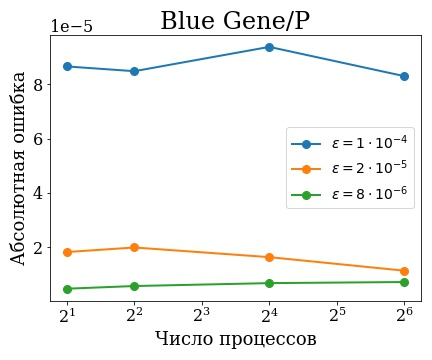
\includegraphics[width=\linewidth]{bluegene_err.jpg} 
        \caption{}\label{fig:bg_err}
    \end{subfigure}
    \hfill
    \begin{subfigure}[t]{0.45\textwidth}
        \centering
        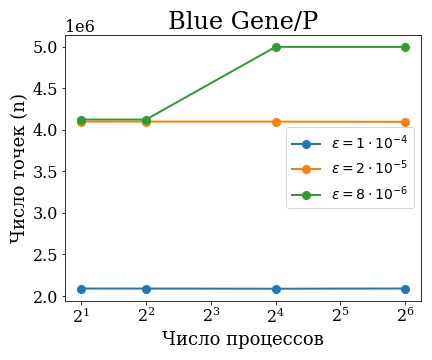
\includegraphics[width=\linewidth]{bluegene_n.jpg} 
        \caption{}\label{fig:bg_n}
    \end{subfigure}
    \medskip
    \begin{subfigure}[t]{0.45\textwidth}
    \centering
    \vspace{0pt}
        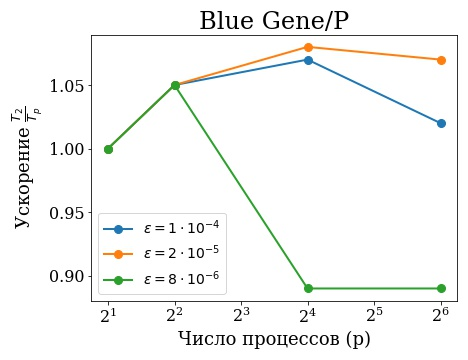
\includegraphics[width=\linewidth]{bluegene_speed.jpg} 
        \caption{}\label{fig:bg_s}
    \end{subfigure}
    \hfill
    \begin{minipage}[t]{.45\textwidth}
    \caption{Сравнение получаемых характеристик запусков на Blue Gene/P \\(абсолютная ошибка -- \subref{fig:bg_err}, \\ число требуемых точек для достижения точности -- \subref{fig:bg_n},\\ ускорение относительно запуска на 2-х процессах -- \subref{fig:bg_s})}
    \label{fig:bg}
    \end{minipage}
    
\end{figure}

\textbf{На Polus}
\begin{itemize}
    \setlength{\itemsep}{1pt}
  \setlength{\parskip}{0pt}
  \setlength{\parsep}{0pt}
 \item Не видна зависимость точности (по абсолютной ошибке) от числа точек. Для оценки данной зависимости также недостаточно приведённых данных.
 \item График ускорения показывает странное поведение для $\varepsilon=5 \cdot 10^{-6}$. Однако данное поведение возспроизводилось на нескольких запусках. Объяснить этот эффект можно запуском на удачных точках, позволяющих оценить интеграл с данной точностью. Поскольку выбирается сразу достаточно точек, то один процесс справляется с задачей вычисления быстрее, чем б\'{ольшее} число.
 \item На системе Polus видна обратная зависимость по ускорению на б\'{о}льшем числе узлов. С ростом числа процессов ускорение растёт (см. график \ref{fig:pl_s}). Этот эффект  может объясняться более эффективной топологией при взаимодействии <<мастера>> с <<рабочими>>.
\end{itemize}

\begin{figure}[ht!]
    \centering
    \begin{subfigure}[t]{0.45\textwidth}
        \centering
        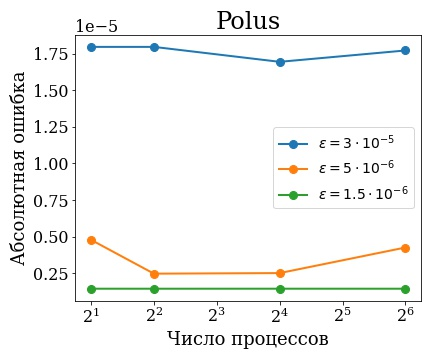
\includegraphics[width=\linewidth]{polus_err.jpg} 
        \caption{}\label{fig:pl_err}
    \end{subfigure}
    \hfill
    \begin{subfigure}[t]{0.45\textwidth}
        \centering
        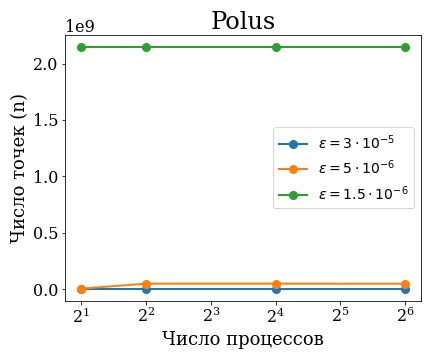
\includegraphics[width=\linewidth]{polus_n.jpg} 
        \caption{}\label{fig:pl_n}
    \end{subfigure}
    \medskip
    \begin{subfigure}[t]{0.45\textwidth}
    \centering
    \vspace{0pt}
        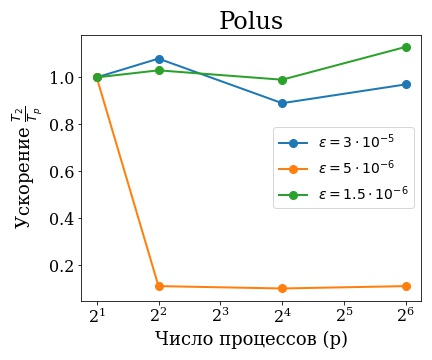
\includegraphics[width=\linewidth]{polus_speed.jpg} 
        \caption{}\label{fig:pl_s}
    \end{subfigure}
    \hfill
    \begin{minipage}[t]{.45\textwidth}
    \caption{Сравнение получаемых характеристик запусков на Polus \\(абсолютная ошибка -- \subref{fig:pl_err}, \\ число требуемых точек для достижения точности -- \subref{fig:pl_n},\\ ускорение относительно запуска на 2-х процессах -- \subref{fig:pl_s})}
    \label{fig:pl}
    \end{minipage}
\end{figure}

\section{Заключение}
В ходе экспериментов с реализацией не выявлено каких-либо существенных закономерностей по точности вычисления. Однако на приведённых графиках можно отследить различие архитектур Blue Gene/P и Polus. 

Также можно отметить, что приведённые результаты не показывают значимых различий из-за попытки задать оптимальное (с некоторой теоретической стороны) начальное число точек. При меньшем числе точек скорости выполнения имели бы более существенные отклонения.
\newpage
\section{Литература}
\begin{thebibliography}{}

\bibitem{Bahvalov97} Бахвалов Н.С., Жидков Н.П., Кобельков Г.М. ЧИСЛЕННЫЕ МЕТОДЫ. - М.: Наука, 1987.
 
\end{thebibliography}
\newpage
\section{Приложение 1. Код программы}\label{sec:code}
\lstinputlisting[language=C, style=customc, label={code:list1}]{../code/mc_master_slave.c}{}

\end{document}
